% !TEX program = xelatex
\documentclass{article}
\usepackage{/Users/jay/LaTeX/cs}
\usepackage{xeCJK}

\newcommand{\hmwkClass}{Artificial Intelligence, Spring 2018}
\newcommand{\hmwkTitle}{Homework 3}
\newcommand{\hmwkDueDate}{May 15, 2018}
\newcommand{\tb}{\textbf}

\begin{document}

\thispagestyle{empty}
\section*{\hmwkClass \\
    \normalsize{\hmwkTitle} \\
    \normalsize{DUE DATE: \hmwkDueDate}
}

\hfill{B03902129 \, 資工四 \, 陳鵬宇}

\section{Problem Formulation}

Please define the Go game's (19*19) states, actions, branching factor and transition model. \\
\textit{hint: follow the definition of 'brancing factor' on the textbook.}

\begin{itemize}
    \item \tb{States:} The board size of the Go is $19 \times 19$, and each intersection can be "empty", "black", or "white", so there are $3^{19 \times 19}$ states in the board. Let $e$ denote "empty", $b$ denote black, and $w$ denote "white".

        The states are $\{\{eee \cdots e\}, \{bee \cdots e\}, \{wee \cdots e\}, \cdots, \{www \cdots w\}\}$.

    \item \tb{Actions:} 
    The actions are $PlayBlack$, $PlayWhite$, and $Pass$.

    There are two players in a Go game. Black player goes first. When it is their turn, a player may either pass (by announcing "pass" and performing no action) or play the color he/she own.
    
    Step 1. (Playing a stone) Placing a stone of their color on an empty intersection.

    Step 2. (Capture) Removing from the board any stones of their opponent's color that have no liberties.

    Step 3. (Self-capture) Removing from the board any stones of their own color that have no liberties.

    Each action may remain the same state ($Pass$) or lead to a new state ($PlayBlack$ or $PlayWhite$).

    \item \tb{Branching factor:} $b = 19 \times 19$.

    \item \tb{Transition model:} Returns the board with the same state, or with a $black$ or $white$ stone added to the specified intersection.

\end{itemize}

\section{Alpha-Beta Pruning}

\begin{figure}[h] 
    \begin{center}
        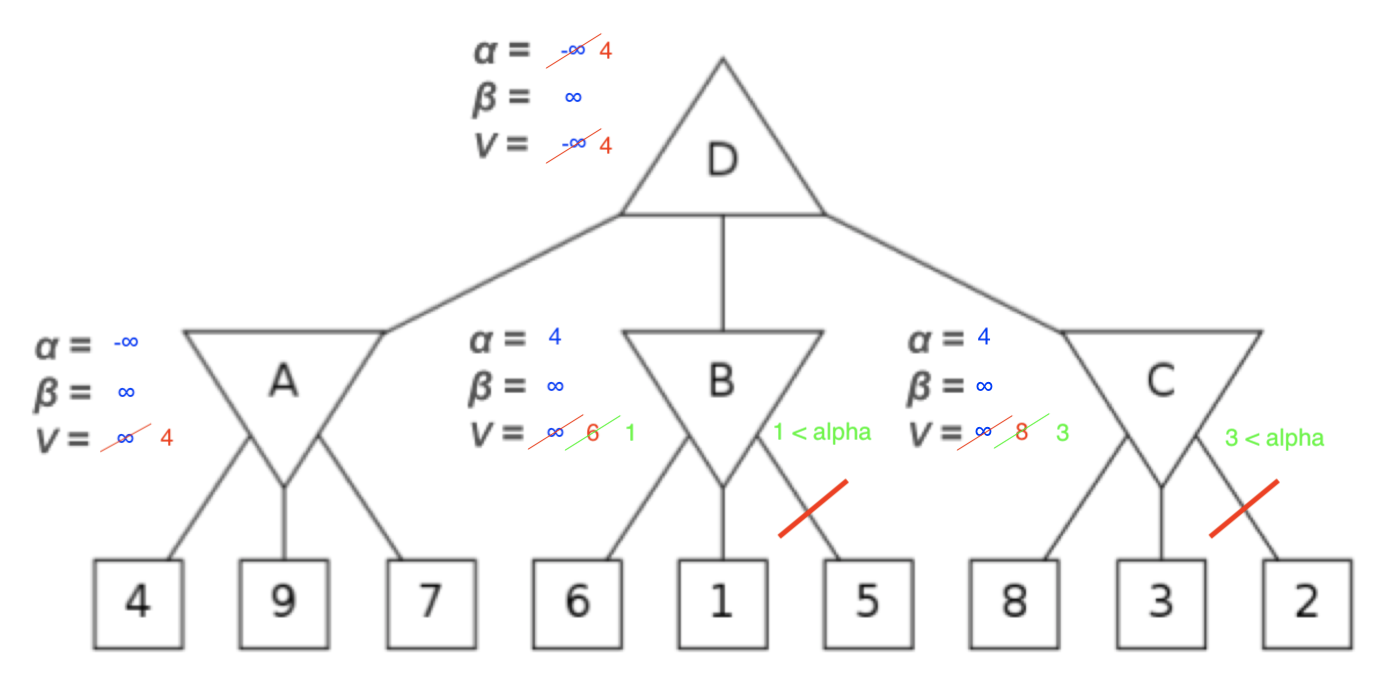
\includegraphics[width=0.8\textwidth]{img/alphaBeta.png} 
    \end{center}
\end{figure}

\newpage

\section{MDP}

\begin{enumerate}[label=(\alph*)]
    \item What is the optimal value $V^*(A)$? Justify your answer briefly.
    % The optimal value of $V^*(A)$ is going $Right$ until $Exit$ state with reward $= 10$ since if we go $Left$ we will exit immediately with reward $= 10$. Furthermore, there is no reason to go $Right$ then $Left$ or to go $Left$ then go $Right$. Since the $Exit$ states are in the leftmost and rightmost position. Thus

    By MDP with $\gamma = 1$, we have the following table:

    $$
    \begin{array}{|l|c|c|c|c|c|}
        \hline
              & +1 &  A &    &    & +10 \\
        \hline
        k = 0 &  0 &  0 &  0 &  0 &   0 \\
        \hline
        k = 1 &  1 &  0 &  0 &  0 &  10 \\
        \hline
        k = 2 &  1 &  1 &  0 & 10 &  10 \\
        \hline
        k = 3 &  1 &  1 & 10 & 10 &  10 \\
        \hline
        k = 4 &  1 & 10 & 10 & 10 &  10 \\
        \hline
    \end{array}
    $$

    $V^*(A) = 10$.

    \item What is the first iteration $k$ for which $V_k(A)$ will be non-zero?

    Because $V_2(A) = 1 \ne 0$, $k = 2$.
    \item What will $V_k(A)$ be when it is first non-zero?

    $V_2(A) = 1$.

    \item After how many iterations $k$ will we have $V_k(A) = V^*(A)$?

    Because $V_4(A) = 10 = V^*(A)$, $k = 4$.

    \item If $\gamma = 0.5$, what is the optimal value $V^*(A)$? Justify your answer briefly.

    By MDP with $\gamma = 0.5$, we have the following table:

    $$
    \begin{array}{|l|c|c|c|c|c|}
        \hline
              & +1  &     A &      &     & +10 \\
        \hline
        k = 0 &   0 &     0 &    0 &   0 & 0 \\
        \hline
        k = 1 & 0.5 &     0 &    0 &   0 & 5 \\
        \hline
        k = 2 & 0.5 &  0.25 &    0 & 2.5 & 5 \\
        \hline
        k = 3 & 0.5 &  0.25 & 1.25 & 2.5 & 5 \\
        \hline
        k = 4 & 0.5 & 0.625 & 1.25 & 2.5 & 5 \\
        \hline
    \end{array}
    $$

    $V^*(A) = 0.625$.

    \item For what range of values $\gamma$ of the discount will it be optimal to go $Right$ from $A$?

    \begin{align*}
        \gamma^2 \cdot 1 & \le \gamma^4 \cdot 10 \\
                \gamma^2 & \ge \frac{1}{10} \\
                \gamma   & \ge \frac{1}{\sqrt{10}}.
    \end{align*}

    \item Let's assume that the $Left$ and $Right$ movement actions are now stochastic and failwith probability $f$. When an action fails, the agent stays in place. The $Exit$ action does not fail. If the failure probability is $f = 0.5$ and the discount $\gamma = 1$, what is the optimal value $V^*(A)$? Justify your answer briefly.

    Since $\gamma = 1$, the failure doesn't affect the $V^*(A)$, the optimal value is still $10$.
\end{enumerate}

\end{document}